\documentclass[12pt]{article}
\usepackage{amsmath,amssymb,amsthm}
\usepackage{microtype}
\usepackage[a4paper,margin=2cm]{geometry}
\usepackage{vwcol} 
\usepackage{lipsum,multicol}
\usepackage[colorlinks]{hyperref} 
\usepackage{caption}
\usepackage{pgfplots}
\usepackage{graphicx}
\usepackage{subcaption}
\usepackage{tikz}
    \usetikzlibrary{positioning}

\setlength\parindent{0pt}
\DeclareMathOperator{\E}{\mathbb{E}}

\tikzset{basic/.style={draw,fill=white,text width=1em,text badly centered}}
\tikzset{input/.style={basic,circle}}
\tikzset{weights/.style={basic,rectangle}}
\tikzset{functions/.style={basic,circle,fill=white}}

\title{CS4243 Computer Vision}

\date{AY2019/20 Semester 1}
\author{Choong Wey Yeh}

\begin{document}

\maketitle

\section{Image Processing}

\subsection{Bayer Filter}
Light passes through the Bayer Filter to capture an image in RGB colours. \\

\begin{figure}[ht]
\begin{minipage}[t]{0.3\linewidth}
\centering
$ \begin{bmatrix} R&G\\ G&B \end{bmatrix}$
\caption*{Bayer Filter Matrix}
\label{GIS_Mapping_Software}
\end{minipage}%
\begin{minipage}[t]{0.7\linewidth}
Local pattern captured by a Bayer Filter. Can be consolidated into a single in multiple ways, the simplest being interpolation. This also known as \textbf{Demosaicing} \\

Demosaicing via interpolation: 
\[
g(x, y) =
\begin{cases}
[R, G, B]_B = [ f(x + 1, y + 1), f(x + 1, y), f(x, y)]\\
[R, G, B]_{GB} = [ f(x, y + 1), f(x, y), f(x - 1, y)]\\
[R, G, B]_{GR} = [ f(x + 1, y), f(x, y), f(x, y - 1)]\\
[R, G, B]_R = [ f(, y), f(x - 1, y), f(x - 1, y - 1)]\\
\end{cases}
\]
\end{minipage}
\end{figure}

\textit{Pixel Intensity} is the grayscale value $I$ given by:
\begin{equation} 
I = W_R \cdot R + W_B \cdot B + W_G \cdot G
\end{equation}
where $W_R, W_B, W_G$ are weights assigned denoting the significance of each colour channel. The standard weights are $W_R = 0.299, W_G = 0.587, W_B = 0.114$.\\

Higher weight is usually given to the green colour channel as it occupies twice as many pixels compared to red and blue.

\subsection{Point Processing}

\textit{Point Processing} refers to image processing techniques that transform a pixel independent of other pixels.

\subsubsection{Brightness and Contrast}

Given a pixel with the original value $p_{ij}$, we can define the new pixel with adjusted brightness and contrast values:
\begin{equation}
p'_{ij} = a \cdot p_{ij} + b = \frac{255}{p_{max} - p_{min}} \cdot p_{ij} + \frac{255}{p_{max} - p_{min}} \cdot (-p_{min})
\end{equation}

where $a$ influences the \textit{contrast} of the pixel, which is the relative difference in intensity to other pixels, while $b$ influences the \textit{brightness}, which is the static intensity level of the image. Using contrast stretching and mean normalization, we can obtain the second form of 
equation (2) above. \\

\subsubsection{Gamma Correction}

Originally used in the past to reflect the original colours of captured images by adjusting the encoded gamma values. The gamma correction equation is as follows:
\begin{equation}
p'_{ij} = 255 \cdot (\frac{p_{ij}}{255})^\gamma, \gamma > 0
\end{equation}

where $\gamma$ is a value that determines the contrast of the image. Higher(> 1) values of $\gamma$ darkens the image, while 
lower values of $\gamma$ brightens.\\

\subsubsection{Logarithmic and Exponential Mapping}

\textbf{Logarithmic Mapping}: Better at normalizing darker pixels(lower intensity value)
\begin{equation}
p'_{ij} = \frac{255}{\log(1 + p_{max})} \cdot \log(1 + p_{ij})
\end{equation}

\textbf{Exponential Mapping}: Better at normalizing brighter pixels(higher intensity value)
\begin{equation}
p'_{ij} = \frac{255}{k^{p_{max}} - 1} \cdot (k^{p_{ij}} - 1), k > 0
\end{equation}

\subsubsection{Histogram Stretching}

Means of normalizing pixel intensity values to make full use of the colour space. 
\begin{equation}
p'_{ij} = p_{ij} \cdot \frac{255}{p_{max} - p_{min}}
\end{equation}

However, histogram stretching does not do so well for histograms with extreme distributions or spiked distributions. Such as in the example figure below, histogram stretching does nothing since there are extreme values at the edge of the intensity spectrum. \\

\begin{figure}[!h]
\centering
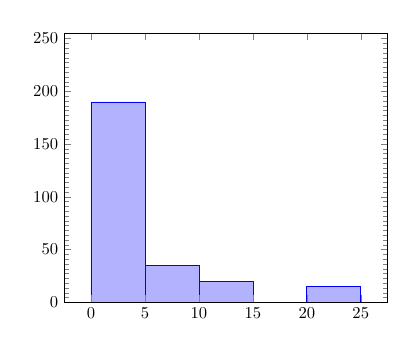
\begin{tikzpicture}[scale=0.6]
\begin{axis}[
    ymin=0, ymax=255,
    minor y tick num = 10,
    area style,
    ]
\addplot+[ybar interval,mark=no] plot coordinates { (0, 190) (5, 35) (10, 20) (15, 0) (20, 15) (25, 165) };
\end{axis}
\end{tikzpicture}
\end{figure}

\subsubsection{Histogram Equalization}

Unlike histogram stretching, histogram equalization smooths the distribution of pixels of an image using probabilistic distribution. Using the cumulative distribution of pixel values in the image, histogram equalization approximates a linear cumulative distribution of pixels over image.\\ 
Let the probability density function of a pixel value $p_{ij}$ be count of pixels of the pixel value $p_{ij}$:
\begin{equation}
p(p_{ij}) = \frac{n_i}{n}
\end{equation}

Then, the cumulative probability distribution(CDF) of pixels is the count of all pixel values less than or equal to that pixel value $p_{ij}$. It gives a percentile and proportion of all pixels that the pixel value $p_{ij}$ occupies. 
\begin{equation}
P(p_{ij}) = \sum p(p_{ij})
\end{equation}

We can use this CDF to approximate the proportion of the intensity spectrum that the pixel should take. That is,
\begin{equation}
p'_{ij} = P(p_{ij}) \cdot 255
\end{equation}

\subsection{Locality Based Processing}

We can process image pixels using information in a window around the pixel, preserving some locality around the pixel. We do this by apply filters. which are processing layers that determine what information is extracted, over image windows using processing techniques.\\

\textbf{Cross-Correlation}: 
\begin{equation}
\sum^k_{u = -k} \sum^k_{v = -k} f_{uv} \cdot P_{i + u, j + v}
\end{equation}

\textbf{Normalized Cross-Correlation}: 
\begin{equation}
\frac{1}{|F||w_{ij}|}\sum^k_{u = -k} \sum^k_{v = -k} f_{uv} \cdot P_{i + u, j + v}
\end{equation}
The processed pixel is normalized by the original pixel value and also the filter values.\\

\textbf{Convolution}: 
\begin{equation}
\sum^k_{u = -k} \sum^k_{v = -k} f_{uv} \cdot P_{i - u, j - v} 
\end{equation}
Convolution is equivalent to flipping the kernel filter and applying cross-correlation. \\
Convolution is mostly used in image processing due to having nice properties, such as associative and distributive properties. The convolution operator is denoted by $\circledast$. \\

\textbf{Linear Separability}: Some kernels can be linearly separated into two or more kernels, and each convolved with the resulting image by the property of association. This allows the operation cost to be reduce from $O(N^2)$ for a $N \times N$ kernel, to $2N$ for $2$ separated kernel filters.

\begin{equation*}
f \circledast I = (
\begin{bmatrix}
1 & 0 & 1\\
3& 0 & 3\\
1 & 0 & 1
\end{bmatrix}) \circledast I = (
\begin{bmatrix}
1\\
3\\
1
\end{bmatrix} \circledast 
\begin{bmatrix}
1 & 0 & 1
\end{bmatrix}) \circledast I = (g \circledast h) \circledast I = g \circledast (h \circledast I)
\end{equation*}

\subsubsection{Gaussian Smoothing}

A common convolution operation that we often use is convolving an image with a gaussian kernel. A gaussian kernel is a filter generated using multivariate gaussian distribution, prioritizing weights in the middle and lowering weights further away from the center. An approximation to the gaussian kernel is as shown below:
\begin{equation}
\frac{1}{16}
\begin{bmatrix}
0 & 1 & 0\\
1& 4 & 1\\
0 & 1 & 0
\end{bmatrix}
\end{equation}

Gaussian smoothing is a low pass filtering technique often used to blur images and remove noise.\\ 
In the actual gaussian kernel formulation, the $\sigma$ term determines the \textbf{extent of smoothing} of the actual gaussian kernel. \\

\subsubsection{Median Filtering}

\textit{Median filtering} is another method of removing noise from image windows by taking the median value of pixels within a window. This prevents large extreme values caused by noise and corruption.\\

\section{Regions \& Boundaries}

\subsection{Edges}

Edges are discontinuities in the image intensity values that help use to identify and determine where boundaries are. Discontinuities are large changes in image intensity values along a certain orientation. To identify large changes in pixel values, we detect the changes via derivatives as in Calculus.\\ 

Using the original definition of derivatives:
\begin{equation}
f'(x) = \lim_{h \rightarrow 0} \frac{f(x + h) - f(x)}{h}
\end{equation} 

Using the central difference alternative:
\begin{equation}
f'(x) = \lim_{h \rightarrow 0} \frac{f(x + 0.5 h) - f(x - 0.5 h)}{h}
\end{equation} 

Taking finite discrete differences, we can approximate the changes for small shift in pixels using the following equation:
\begin{equation}
f'(x) =  \frac{f(x + 1) - f(x - 1)}{2}
\end{equation} 

From equation (16), we can formulate 1 dimensional derivative filters: 
\begin{figure}[!ht]
\begin{equation}
\begin{bmatrix}
-1 & 0 & 1\\
\end{bmatrix}
\end{equation}
\caption{1 dimensional horizontal derivative filter}
\end{figure} 

However, differentiation and derivatives by itself accentutates noise in images due to the large anomalies and extreme values of noisy pixels. Hence before we apply derivative filters, we often smooth the images (e.g gaussian smoothing) to reduce noise.

\begin{flalign} 
\begin{aligned}
\frac{\delta}{\delta x} (h \circledast I) &= 
\begin{bmatrix}
-1 & 0 & 1\\
\end{bmatrix} \circledast 
( \begin{bmatrix}
1 \\
2 \\
1 \\
\end{bmatrix} \circledast I) \hspace{10mm} \text{using} \begin{bmatrix}
1 \\
2 \\
1 \\
\end{bmatrix} \text{as 1D approximate gaussian filter} \\
&= (\begin{bmatrix}
-1 & 0 & 1\\
\end{bmatrix} \circledast 
\begin{bmatrix}
1 \\
2 \\
1 \\
\end{bmatrix} ) \circledast I \hspace{10mm} \text{using associative property of convolution} \\
& = 
\begin{bmatrix}
-1 & 0 & 1\\
-2 & 0 & 2\\
-1 & 0 & 1\\
\end{bmatrix} \circledast I = (\frac{\delta}{\delta x} \circledast h) \circledast I 
\end{aligned}&&&
\end{flalign}

Here, we use the associative property of convolution to convolve the derivative filter with an approximate gaussian filter to produce the horizontal Sobel filter.

\begin{figure}[!h]
\begin{minipage}[t]{0.5\linewidth}
\centering
\begin{equation*}
f_x = 
(\begin{bmatrix}
-1 & 0 & 1\\
\end{bmatrix} \circledast 
\begin{bmatrix}
1 \\
2 \\
1 \\
\end{bmatrix} ) = 
\begin{bmatrix}
-1 & 0 & 1\\
-2 & 0 & 2\\
-1 & 0 & 1\\
\end{bmatrix}
\end{equation*}
\caption*{Horizontal Sobel Filter: Detects vertical edges}
\end{minipage}
\begin{minipage}[t]{0.5\linewidth}
\centering
\begin{equation*}
f_y = 
(\begin{bmatrix}
1 & 2 & 1\\
\end{bmatrix} \circledast 
\begin{bmatrix}
1 \\
0 \\
-1 \\
\end{bmatrix} ) = 
\begin{bmatrix}
1 & 2 & 1\\
0 & 0 & 0\\
-1 & -2 & -1\\
\end{bmatrix}
\end{equation*}
\caption*{Vertical Sobel Filter: Detects horizontal edges}
\end{minipage}
\end{figure}

\textbf{Gradient vector}: $\triangledown f = [\frac{\delta f}{\delta x} = f_x \circledast I = I_x, \frac{\delta f}{\delta y} = f_y \circledast I = I_y] $\\

\textbf{Orientation of gradient}: $\theta = \tan^{-1} \frac{I_x}{I_y}$\\

\textbf{Gradient magnitude}: $|\triangledown f | = \sqrt{I_x^2 = I_y^2}$

\section{Canny Edge Detection}

Canny Edge Detection is a framework for detecting edges accurately in images. It first extracts the image derivatives using convolution, which are used to determine edge locations. Edges are then thresholded, and weak edges are linked using hysterisis thresholding.
\begin{enumerate}
\item Obtain image derivatives by applying derivative filters over the image using convolution. We preserve the \textbf{gradient magnitude} $|\triangledown f |$ and \textbf{gradient angle} $\theta$ for later phases of the Canny Edge Detection framework.

\item Apply \textbf{Non-Maximum Suppression} to thin out edges. Obtaining the gradient magnitudes may result in some visualised edges having thicker boundaries than others if the edge has high contrast or gentle descent gradients. 
\begin{itemize}
\item For each pixel, we follow the gradient orientation along the dominant direction using the gradient angle $\theta$, and pick the pixel with the locally maximal value along that path.
\item We suppress all other values along the same trajectory by setting the gradient magnitude values to 0. This gives consistent edge width for all edges detected.
\end{itemize}

From the previous 2 steps of the edge detection algorithm, we would have extracted the primary edges in the image. However, many edges that are weak, or edges that slowly diminish in discontinuity differences may be lost. Hence, we need to reconnect these edges using \textbf{Hysterisis Thresholding}.\\

\subsection{Hysterisis Thresholding}

\item We define 2 thresholds, a \textbf{high} and \textbf{low} threshold. We use the high threshold to identify strong edges, which will be our main boundaries in the image, while the low threshold identifies weak edges.
\item We start from each strong edge, and \textbf{iteratively add pixels which are part of weak edges but also connected to strong edges}. This allows to perform \textbf{linking} of weak edges to strong edges to continue them.

\end{enumerate}

\section{Regions and Contours}

We can easily identify objects by identifying the boundaries that segment objects, and properties in the regions of images. \\

Similar objects and textures have similar properties and characteristics in the form of pixel and colour intensity and patterns.By identifying these similarities, we can group like objects together through similar pixels in order to accentuate and isolate objects in the image. One way that we can achieve this is to define clusters and assign pixels to their appropriate clusters through clustering techniques.

\subsection{Image Segmentation}

\subsection{K-Means Clustering}

The K-Means clustering algorithm aims to define clusters of data points for $k$ clusters by defining the \textbf{cluster centroid} for the $i^{th}$ cluster, $\mu_i$. Here, the hyperparameter $k$ is a inductive learning bias that we must decide and tune.\\

\subsubsection{Expectation Maximization Algorithm}
The algorithm is based on the Expectation Maximization(EM) algorithm using Bayesian probabilistic heuristics. Given $D$ data points that are assumed to be generated by a gaussian distribution(the assumption of gaussian is not too bad given the Central Limit Theorem if $D$ is large), we aim to estimate that for $k$ gaussian distribution, the collection of parameters that is the means of each of the gaussians $\mu_1,..., \mu_k$ such that each data point is generated by a $j^{th}$ gaussian that maximizes the maximum likelihood estimate(MLE).\\

Given the participation constraints for the $i^{th}$ data points $d_i$, we aim to maximize the expected participation, or the probability that the $j^{th}$ gaussian generates $d_i$:
\begin{equation*}
\text{argmax} \E [z_{ij}] = \text{Pr} (z_{ij} | d_i) = \frac{\exp(-\frac{1}{2 \sigma^2} (d_i - \mu_i)^2)}{\sum_{k=1}^{m} \exp(-\frac{1}{2 \sigma^2} (d_i - \mu_k)^2)}
\end{equation*}

Clearly, we can see that the expectation above is maximized when the distance between the data point $d_i$ and the mean of the generating gaussian $\mu_j$ is minimized. In particular, for a set of data points $D$ and parameters containing the means of the gaussians $h = \{ \mu_1, ..., \mu_m \}$, we want to find the hypothesis that maximizes the following MLE:
\begin{equation}
\text{argmax} \E[\log (p(D|h))]
\end{equation} 

Performing the derivative, we have that the update step is: 
\begin{equation}
\mu'_j = \frac{\sum_{d \in D} \E]z_{ij}] d_i}{\sum_{d \in D} \E]z_{ij}]}
\end{equation}

Hence, to find the centroid clusters $\mu_j$, the algorithm is as follows:\\

Randomly initialize $m$ cluster centroids.
For each iteration, assign each point to the nearest cluster centroid. This is the expected cluster centroid that produces $d_i$.
\begin{equation}
z_i = \text{argmin}_{j} |p_i - c_j|^2
\end{equation}

where $z_i$ denotes the gaussian that generates the $i^{th}$ point. Then, we re-estimate each cluster centroid until convergence:
\begin{equation}
c_j = \frac{\sum_{i; y_i = j} p_i}{\sum_{i; y_i = j} 1}
\end{equation}

However, K-Means algorithm is:
\begin{enumerate}
\item Highly sensitive to the initial cluster centroids generated
\item Effectiveness depends on the correct $k$ selected, which is usually not trivial
\end{enumerate}

\subsection{Mean Shift Clustering}

Unlike K-Means algorithm, Mean-Shift algorithm is a mode finding algorithm that finds centroid clusters based on the probability density function of the distribution of points. This means that Mean-Shift is able to model black-box probability density functions instead of assuming gaussian distribution like in K-Means.\\

Given $n$ points, the multivariate kernel estimate with mean $x$ is
\begin{equation}
f_k(x) = \frac{1}{nh^d} \sum^n_{i=1} K(\frac{x - x_i}{h})
\end{equation}

where $h$ is the bandwidth parameter, which specifies the kernel density window and $K$ the kernel function(Epanechikhov, Gaussian). For example, we may use the Gaussian Kernel(in probability) to denote our kernel function, which has higher value when distance between 2 points is small. Again taking the derivative to maximize MLE of the above probability density function, we have that:
\begin{equation}
\text{argmax}_x f_k(x_i) \rightarrow \triangledown f_k(x_i) = \alpha [\sum_{i=1}^n g(|\frac{x-x_i}{h}|^2)] [\frac{\sum_{i=1}^n g(|\frac{x-x_i}{h}|^2) x_i}{\sum_{i=1}^n g(|\frac{x-x_i}{h}|^2)} - x] = 0
\end{equation}

where the middle term $[\sum_{i=1}^n g(|\frac{x-x_i}{h}|^2)$ is the current kernel density estimate. We want to maximize the probaility density function by taking the gradient vector equals to zero. Since the current kernel density estimate is not equal to zero(unless there are no points), we have that we must have $\frac{[\sum_{i=1}^n g(|\frac{x-x_i}{h}|^2) x_i}{[\sum_{i=1}^n g(|\frac{x-x_i}{h}|^2)} - x = 0$, and hence the new mean $x' = \frac{\sum_{i=1}^n g(|\frac{x-x_i}{h}|^2) x_i}{\sum_{i=1}^n g(|\frac{x-x_i}{h}|^2)}$. Here, $\frac{\sum_{i=1}^n g(|\frac{x-x_i}{h}|^2) x_i}{\sum_{i=1}^n g(|\frac{x-x_i}{h}|^2)} - x$ is known as the mean-shift vector.\\

Using the kernel density in a window, the Mean-Shift algorithm is able to approximate the probability density function by taking histograms of projected kernel densities. However, the downfall of Mean-Shift algorithm is that:
\begin{enumerate}
\item Bandwidth parameter $h$ is not trivial to tune
\item Slow to converge
\end{enumerate}

\subsection{Textures}

Textures refers to the outward appearance of a specific object. The appearance may bestow properties and characteristics that help us to distinguish between objects. Texture on objects are made out of local repeating patterns, known as textons. We can identify these textons, and group similar patterns together to the same texton.

\subsubsection{Filter Bank}

One way to identify textures and textons is through the use of filters. Similar textons will produce similar responses to the same set of filters, and hence like textures will have similar textons. To identify and obtain these textons, we first formulate a set of filters used to test for responses from image patches known as the \textbf{filter bank}. The filter bank consists of multiple filters that should be carefully selected to extract meaningful information from texture patches. \\

For a filter bank with $d$ filters, we can obtain the responses of an image patch for each filter, forming a $d$ dimensional fixed vector representation. We can perform this routine for each of the images in a training dataset, obtaining feature vectors that represent different textons and textures in our training data.\\ 

\subsubsection{Texture Segmentation}
In order to perform texture segmentation, again we need to identify key texton descriptions. Using a filter bank, we may obtain various feature vectors representing different textons. However, in order to obtain meaningful representations of textons, we performing clustering just as in the previous section on the texton feature vectors obtained from our training set using our filter bank, and the centroid clusters will form our textons.\\

With these centroids, we can then replace each pixel in an image by applying our filter bank on it, and then binning the response vector to the nearest centroid. Since like textures will have similar repeating textons, and hence produce similar responses, they will have the same texton assigned to it in the segmented image, allowing us to isolate and identify different textures in images. To obtain a representation of texture, we can then take a histogram of textons in a local patch of an image.

\subsubsection{Comparing Histograms}

To compare histogram(vectors) of textures, we need a distance metric to compare them. Since they are in vector form, the euclidean($l_2$) distance is easiest to use. However, it does not take into account the relative coordinates between histograms.\\

\textbf{$\chi^2$ Distance}: $\sum_I \frac{(H_1(I) - H_2(I))^2}{H_1(I)}$ \\
Takes into account the relative coordinates of vectors\\ 

\textbf{Bhattacharyya Distance}: $\sqrt{1 - \frac{1}{\sqrt{H_1H_2N^2}} \sum\sqrt{H_1(I) - H_2(I)}}$ \\
Similar to $\chi^2$, but non-symmetric

\section{Local Features}

Local features are keypoints in an image that identify a specific feature through it's local surrounding pixels.

\subsection{Characteristics of a good local feature}
\begin{enumerate}
\item \textbf{Repeatability}: Ability to find the same points in different images, despite translation and transforms of the image.
\item \textbf{Distinctive}: Properties that identify this feature should not be widely common with other features.
\item \textbf{Efficient}: Extracting information from the local window should not be heavy, and representation should be of limited size.
\item \textbf{Local}: Captures information from a small window around the feature
\end{enumerate}

\subsubsection{Aperture Problem}

The aperture problem is where changes in the image are not detected due to the locality of the window itself being too restricted, or the feature itself lacking distinctiveness. Hence, we want to choose features that are unique such that small changes in all directions from the current feature window. will result in a large change in the intensity distribution.

\begin{figure}[!htb]
\centering
  \includegraphics[width=80mm]{aperture.jpg}
  \caption{Aperture Problem Visualisation}
  \label{fig:AP}
\end{figure}

\subsection{Corner Detection}
Previously, we mentioned that good features must be unique, and respond to changes in all directions of the image. Thus, we can use corners as a good feature. Consider a small shift of displace $(u, v)$  from the initial position $(x, y)$. Then, the sum of squared differences(SSD) of the shift can be formulated as:
\begin{flalign}
\begin{aligned}
E(u, v) &= \sum_{(x, y) \in W} [I(x + u, y + v) - I(x, y) ]^2 \\
& = \sum_{(x, y) \in W)} [I(x + y) + \triangledown I \cdot \triangle(u ,v) + I(x, y)]^2\ \text{using Taylor's 1st order approximation} \\
&= \sum_{(x, y) \in W} [\frac{\delta I}{\delta x}u + \frac{\delta I}{\delta y}v]^2 = \sum_{(x, y) \in W} [I_xu + I_yv]^2
\end{aligned}
\end{flalign}

where we approximate the changes in the pixel intensity at the current position $(x ,y)$ with a displace of $(u, v)$. We can further decompose the equation using Singular Value Decomposition (SVD), into:

\begin{flalign}
\begin{aligned}
E(u, v) &= \sum_{(x, y) \in W} [I_xu + I_yv]^2 \\
&= \sum_{(x, y) \in W} I_x^2u^2 +  \sum_{(x, y) \in W} I_xI_yuv +  \sum_{(x, y) \in W} I_y^2v^2 \\
& =  \begin{bmatrix}
u & v\\
\end{bmatrix}
\begin{bmatrix}
\sum_{(x, y) \in W} I_x^2 & \sum_{(x, y) \in W} I_xI_y\\
\sum_{(x, y) \in W} I_xI_y & \sum_{(x, y) \in W} I_y^2\\
\end{bmatrix} 
\begin{bmatrix}
u\\
v\\
\end{bmatrix}
&= \begin{bmatrix}
u & v\\
\end{bmatrix}
H
\begin{bmatrix}
u\\
v\\
\end{bmatrix}
\end{aligned}
\end{flalign}

where $H$ is the Hessian matrix, or second moment matrix. Furthermore, since $H$ is positive definite symmetric, we can decompose the $H$ matrix into it's eigenvectors and eigenvalues using orthogonal diagonalization: 

\begin{flalign}
\begin{aligned}
E(u, v) &=  \begin{bmatrix}
u & v\\
\end{bmatrix}
\begin{bmatrix}
\sum_{(x, y) \in W} I_x^2 & \sum_{(x, y) \in W} I_xI_y\\
\sum_{(x, y) \in W} I_xI_y & \sum_{(x, y) \in W} I_y^2\\
\end{bmatrix} 
\begin{bmatrix}
u\\
v\\
\end{bmatrix} \\
&= \begin{bmatrix}
u & v\\
\end{bmatrix}
H
\begin{bmatrix}
u\\
v\\
\end{bmatrix} \\
&= \begin{bmatrix}
u & v\\
\end{bmatrix}
\begin{bmatrix}
v_{\lambda_1} & v_{\lambda_2}\\
\end{bmatrix}
\begin{bmatrix}
\lambda_1 &0\\
0 & \lambda_2 \\
\end{bmatrix}
\begin{bmatrix}
v_{\lambda_1}\\
v_{\lambda_2}\\
\end{bmatrix}
\begin{bmatrix}
u\\
v\\
\end{bmatrix} \\
\end{aligned}
\end{flalign}

where $\lambda_1$ and $\lambda_2$ corresponds to the respective changes along the 2 eigenvectors $v_{\lambda_1}$ and $v_{\lambda_2}$. More specifically, in this case the magnitude of $\lambda_1$ and $\lambda_2$ corresponding directly to changes in the $x$ and $y$ directions, $I_x$ and $I_y$. High values of $\lambda_1$ corresponding to a large $I_x$ value, and indicates a strong change in the $x$ direction from a small displace $(u, v)$. The same argument applies for the $y$ direction as well.\\

Hence, we can use the eigenvalues from SVD of the matrix to obtain the 'cornerness' score of the image patch. A naive way of doing this is to take the minimum eigenvalue, and threshold it.\\

\textbf{Kanade \& Tomasi}: $R = \min(\lambda_1, \lambda_2)$
However, this cornerness function accounts only for one eigenvalue instead of both. We want a function that derives scores from both eigenvalues $\lambda_1$ and $\lambda_2$. The following 2 scoring functions are better at deriving cornerness scores from eignevalues.\\

\textbf{Harris}: $R = \det(H) - \kappa tr^2(H)$\\
\textbf{Nobel}: $R = \frac{\det(H)}{tr(H) + \epsilon}$\\

Note that since $H$ is positive definite symmetric, then we have that:
\begin{flalign}
\begin{aligned}
\det(H) &= \det(
\begin{bmatrix}
v_{\lambda_1} & v_{\lambda_2}\\
\end{bmatrix}
\begin{bmatrix}
\lambda_1 &0\\
0 & \lambda_2 \\
\end{bmatrix}
\begin{bmatrix}
v_{\lambda_1}\\
v_{\lambda_2}\\
\end{bmatrix}
) \\
&= \det(
\begin{bmatrix}
v_{\lambda_1} & v_{\lambda_2}\\
\end{bmatrix}
\begin{bmatrix}
v_{\lambda_1}\\
v_{\lambda_2}\\
\end{bmatrix}
\begin{bmatrix}
\lambda_1 &0\\
0 & \lambda_2 \\
\end{bmatrix}
)\\
&= det(\begin{bmatrix}
\lambda_1 &0\\
0 & \lambda_2 \\
\end{bmatrix}) = \lambda_1\lambda_2
\end{aligned}
\end{flalign}

In general, we prefer the use of the Nobel and Harris corner detection functions because we can derive the cornerness scores without having to explicitly compute the eigenvalues, which can be rather expensive, as we have to do in Kanade \& Tomasi. But even then, Kanade \& Tomasi's method finds a good approximation of the corner space through thresholding(by only taking regions where both axes has sufficient change).\\

Since $v_{\lambda_1} \& v_{\lambda_2}$ are orthonormal vectors, and hence the matrices are invertible.\\

Another thing to note is that taking gradients in a simple window does not account for spatial layout of the image, and hence such information is not incorporated into the above cornerness functions. To mitigate this, we can introduce a weighting mechanic similar to that used in the gaussian kernel where the $H$ matrix is now: $ \sum_{(x, y) \in W} w_{x,y} \begin{bmatrix}
\sum_{(x, y) \in W} I_x^2 & \sum_{(x, y) \in W} I_xI_y\\
\sum_{(x, y) \in W} I_xI_y & \sum_{(x, y) \in W} I_y^2\\
\end{bmatrix} $ such that the weight $w_{x, y}$ is lower the further away the pixel is form the center of the window.

\subsubsection{Corner Detection Algorithm}

The basis corner detection algorithm using the corner formulation score above is as follows:

\begin{enumerate}
\item Compute gradients of the image using convolution with derivative filters to obtain the $I_x$ and $I_y$ matrix. 
\item Compute the Hessian matrix $H$ for each window, and apply the selected cornerness function(e.g Harris) on the $H$ matrix to obtain the cornerness score.
\item Threshold cornerness function score values for obtained responses.
\item Apply Non-Maximum Suppression to retrieve the local maxima. Basic NMS may be vulnerable to interest points in areas of higher contrast. We can use Adapative NMS to only pick features that are local maxima and also with cornerness scores 10\% higher than it's neighbours. 
\end{enumerate}

\subsection{Feature Description Properties}

For a specific image transformation, we say that for a corner is:\\

\textbf{Invariant} if corner locations remain unchanged in transformed images.\\

\textbf{Equivariance} if corner locations are detected in the corresponding locations after transformation.\\

We want corners to be:\\

\begin{itemize}
\item \textbf{Invariant} to photometric transformations(brightness and contrast changes)
\item \textbf{Equivariant} to geometric transformations(translation and affine transforms)
\end{itemize}

Harris corners are \textbf{equivariant} to translation since derivatives via image convolution changes accordingly with the translated image in terms of orientation. Additionally, the magnitude of the gradients do not change, and hence the eigenvalues are the same. The corner response is hence \textbf{invariant} to translation.  However, Harris corners are \textbf{not invariant/equivariant to scaling} since the same location in the original image may be detected as different multiple corners in the new image.\\

Given the linear intensity equation $p'_{ij} = a \cdot p_{ij} + b$, Harris corners are \textbf{invariant} to constant changes in brightness(change in $b$). However, it is \textbf{not invariant} to changes in contrast(changes in $a$) as the derivatives would also be scaled by a factor of $a \rightarrow aI_x, aI_y$ and hence the $H$ matrix and the corner response would be scaled quadratically, increasing the tendency to detect corners.

\subsection{Automatic Scale Detection}

Sometimes the scale of the image greatly impacts the effectiveness of corner detection. If the image is too zoomed in, then it may only capture a fraction of the corner and not detect it. Consequently, zooming out may result in the algorithm detecting the wrong corners. We can introduce detection over multiple scales to obtain the best scale which the corner response for that window is that highest. The set of images of different scales are also called \textbf{Image Pyramids}.\\

\textbf{NOTE:} Often scaling the window may disrupt certain intricate properties of the detection algorithm or descriptor we use, and it's hence safer to scale the image instead.\\

\subsubsection{Laplacian of Gaussian(LoG)} 

An example of multiscale detection is using the Laplacian of Gaussian (LoG) filter. The Laplacian is know as the second derivative in Calculus, and being a type of derivative we can also use it to detect changes and discontinuities. It also works well as a blob detector. Compared to the first derivative filters, which may have large spikes and extreme values in edges if discontinuity is large, the Laplacian filter is able to more precisely capture the edges as it does not have large spikes. Since it's a derivative filter, we again introduce smoothing through gaussian kernel, giving the LoG filter.

\begin{flalign}
\begin{aligned}
\triangledown^2 g(I(x, y)) &= (\triangledown^2) (g(I(x, y))\\
&= \frac{\delta^2 g}{\delta x^2} (I(x, y)) + \frac{\delta^2 g}{\delta y^2} (I(x, y)) \text{By associative property of convolution} \\
&= I_{xx} + I_{yy} = \begin{bmatrix}
1 & -2 & 1\\
\end{bmatrix} \circledast I + 
\begin{bmatrix}
1\\
-2\\
1\\
\end{bmatrix} \circledast I \\
&= ( \begin{bmatrix}
1 & -2 & 1\\
\end{bmatrix} + 
\begin{bmatrix}
1\\
-2\\
1\\
\end{bmatrix}) \circledast I \\
&= ( \begin{bmatrix}
0 & 1 & 0\\
1 & -4 & 1\\
0 & 1 & 0\\
\end{bmatrix} \circledast I
\end{aligned}
\end{flalign}

where $\begin{bmatrix}
0 & 1 & 0\\
1 & -4 & 1\\
0 & 1 & 0\\
\end{bmatrix} $ is the approximate LoG filter as taking derivatives twice of a gaussian can be very expensive. The LoG filter has the highest response as a blob detector when the scale of the image matches similarly to the native scale of the LoG kernel.

\subsection{Feature Descriptors}

After taking our keypoints, such as Harris corners, we need a way to represent and describe the detected keypoints. Previously we mentioned that our representation should be local and compact. In addition to this, we also require that descriptors be \textbf{invariant} to both {photometric and geometric} transformations in order to preserve distinctiveness.\\

Let us first look naive descriptor representations, such as colour histograms and vectorized pixel intensity. By vectorizing the pixel intensity itself, the representation changes largely if we rotate the image, which means it is not invariant to geometric transformations, even if it is normalized to handle photometric transformations. Colour histograms are robust against translations, but do not well against photometric transforms, and do not provide information on shapes and boundaries.\\

\subsubsection{Scale Invariant Descriptors}

Now we shall look at some examples of descriptors that are invariant or at least robust to geometric and photometric transforms.

\paragraph{Multi Scale Oriented Patches(MOPS)}
\begin{itemize}
\item 40 $\times$ 40 window around the selected keypoint.
\item \textbf{Photometric Transform Invariance}: Normalization of pixel intensity by subtraction of mean and division of standard deviation
\item \textbf{Rotation Invariance}: Rotation of patches to canonical orientation By rotating dominant orientation to the right 90 degrees 
\end{itemize}

\paragraph{GIST Descriptor}
\begin{itemize}
\item \textbf{Spatial Layout}: Subsamples the image patch into 4 $\times$ 4 cells, allowing it to encode the spatial layout of filter responses
\item Filter bank of Gabor filters used to obtain responses from the image patch cells. Gabor filters roughly approximate derivatives at a small scale, allowing GIST to encode an approximate spatial layout of gradients and orientations.
\end{itemize}

\paragraph{Scale Invariant Feature Transform(SIFT)}
SIFT is actually a full fledged detection and descriptor framework, consisting of:
\begin{itemize}
\item Multiscale Extrema Detection
\item Keypoint Localization
\item Orientation Assignment
\item Keypoint Description
\end{itemize}

The descriptor for SIFT is formulated as follows:
\begin{enumerate}
\item 16 $\times$ 16 window is taken around the keypoint, and divided further into 4 $\times$ 4 cells
\item For each cell:
\begin{enumerate}
\item Edge orientation of gradients are computed for each pixel
\item Weak edges with low gradient magnitude are thresholded out
\item Surviving gradients are binned according to their edge orientations in 8 cardinal directions.
\end{enumerate}
\item The descriptions for each cell are vectorized and compacted to form 16 $\times$ 8 = 128 dimensional vector.
\end{enumerate}

The SIFT descriptor is descriptive, being able to represent gradients in 8 directions as well as being fast and efficient due to it's local window and compact representation. More importantly, it is robust to scale and rotation through rotation of patch to dominant orientation in Orientation Assignment step, allowing it to have some invariance to geometric transformations.

\section{Feature Matching}

After extracting keypoints from images and representing them as feature descriptors, we are now ready to match features from two different images. Remember that we required that descriptors be distinctive and unique, allowing the same features to be detected in different images, and ahve the same unique representation in both images.\\

In order to match features, we need to define a distance metric like before to determine how close or different a feature vector is to another. Again, we can use euclidean distance as a naive metric, or $\chi^2$ and Bhattacharyya distance metrics. Given the list of feature descriptors in both images, we need to compute and compare the distances between each pair of descriptors, resulting in this operation being quadratic in time complexity.

\subsection{Image Projections}

One of the many uses of feature matching is to provide locations to stitch two images together, like in a panorama. After comparing feature descriptors and picking the set of closest matches, we can stitch them together using the selected keypoints. However, the stitching process may result in images having tears during the mosaicing process. This is because the images may not lie on the same plane. Hence, we need to fix this by applying image projections on the respective images.\\

\subsubsection{Direct Linear Transform}
Currently, our image pixels are in heterogenous coordinates $(x, y)$ which only allows it to be represented in 2 dimensions. In order to perform projective transforms, we need a third coordinate to form homogenous coordinates.\\

First, we transform our hetergoenous coordinates to homogenous ones: $P = \begin{bmatrix}
x\\
y\\
\end{bmatrix} \rightarrow \begin{bmatrix}
x\\
y\\
1\\
\end{bmatrix}$\\

Next we wish to find a linear transformation from our current point $P$ in one image to a point $P'$ in another image: $P' = H \cdot P $. Here $H$ is known as the homography matrix.\\

\text{We expand the linear equation to find each correspondence}

\begin{equation*}
P' = H \cdot P \rightarrow 
\begin{bmatrix}
x'\\
y'\\
1\\
\end{bmatrix} =  \alpha
\begin{bmatrix}
h_1 & h_2 & h_3\\
h_4 & h_5 & h_6\\
h_7 & h_8 & h_9\\
\end{bmatrix}
\begin{bmatrix}
x'\\
y'\\
1\\
\end{bmatrix}
\end{equation*}

Expanding the matrix multiplication, we get that 
\begin{equation*}
x' =\alpha( h_1x + h_2y + h_3 )
\end{equation*}
\begin{equation*}
y' = \alpha(h_4x + h_5y + h_6 )
\end{equation*}
\begin{equation*}
1 = \alpha(h_7x + h_8y + h_9 )
\end{equation*}

Rewriting the equations, we get that 
\begin{equation*}
x'(h_7x + h_8y + h_9 ) = ( h_1x + h_2y + h_3 )
\end{equation*}
\begin{equation*}
y'(h_7x + h_8y + h_9 ) =(h_4x + h_5y + h_6 )
\end{equation*}

Rearranging the terms,
\begin{equation*}
h_7xx' + h_8x'y + h_9x' - h_1x - h_2y - h_3 = 0
\end{equation*}
\begin{equation*}
h_7xy' + h_8yy' + h_9y' - h_4x - h_5y - h_6 = 0
\end{equation*}

Again, we can rewrite into matrix form, for the $i^{th}$ point:
\begin{equation*}
\text{Solve } A_ih = 0 \text{ where}
\end{equation*}
\begin{equation*} A_i =
\begin{bmatrix}
-x & -y & -1 & 0 & 0& 0 & xx' & yx' & x' \\
0 & 0 & 0 & -x & -y& -1 & xy' & yy' & y' \\
\end{bmatrix}
\end{equation*}
\begin{equation*} h = 
\begin{bmatrix}
h_1 & h_2 & h_3 & h_4 & h_5 & h_6 & h_7 & h_8 & h_9 \\
\end{bmatrix}
\end{equation*}

Performing the same routine for each of the keypoints to it's matches, we can get the following equation to solve for the matrix $H$ using SVD(details omitted):
\begin{equation*}
Ah = \begin{bmatrix}
A_1\\
A_2 \\
...\\
A_k\\
\end{bmatrix} h = U\Sigma V^T h =0
\end{equation*}

\subsubsection{DLT Drawbacks}
As seen in the formulatin above, we attempt to find a linear transformation for project our current point into the new point in the other image. However, what if the transformation is not actually linear? Then DLT would result in very bad approximations of the linear transform.\\

Additionally, DLT is very sensitive to bad outliers(bad matches). Having bad matches would result in wrong points being matched and hence bad stitching. We can rectify this with RANSAC.

\subsubsection{Random Sample Consensus(RANSAC}

Random Sample Consensus (RANSAC) aims to iteratively estimate the best model parameters to fit a noisy observation. In our case, our matches may contain bad correspondences. RANSAC iteratively samples a bunch of points from our existing matches, computes the homography matrix $H$ and gets the best $H$ matrix from all the iterations to reduce negative contribution from noisy observations.\\

\textbf{Algorithm:}\\
For each iteration:\\
\begin{itemize}
\item Sample $N$ correspondences randomly from all matched keypoints
\item Compute the homography matrix $H$ using these selected keypoints
\item We define a error threshold $\delta$, and count the number of inlier points $x$ in our keypoints such that $x' - Hx < \delta$
\item If the current homography $H$ produces the largest number of inliers so far, we update the homography matrix $H$ and record the inliers
\end{itemize}
Recompute the homography $H$ again using all inliers captured in our best homography. \\

RANSAC ensures that the homography computed is the best among all the $H$ matrices found through all iterations. More importantly, it keeps the best $H$ matrix influenced by the most inliers and recomputes it at the end using only inliers, which reduces impact of outliers on computing $H$ using DLT.

\section{Recognition}

Image recoginition can be divided into 2 categories: \textbf{Categorical} vs. \textbf{Object} recognition. Categorical recognition is involved with finding a class or subtype of objects, and is generally concerned with identifying generic features relevant to these categories. On the other hand, object or instance recognition is concerned with identifying a specific type of object, and usually deals with very specific features pertaining to that object itself.\\

In particular, it is beneficial to employ dense features such as dense SIFT, which subsamples every $x^{th}$ pixel in the image patch and takes local features around it. This allows the features extracted to be largely representative of the image as a whole, preserving some spatial layout properties.  This is useful when we want to detect classes of objects that may look different, but preserve similar structure.However, dense feature extraction is extremely slow, especially on large images.\\

On the other hand, sparse local features are more specific, and do a better job at identifying specific objects as those features are more likely to be specific to that object itself. Additionally, good feature representations often use some kind of histogram binning to reduce variance and sensitivity to small changes and variations, such binning in 8 cardinal directions in SIFT descriptors.\\

In both cases, recognition tasks themselves can be challenging because of the variations in features for categorical recognition and viewpoints for instance recognition. Other factors such as illumination and occlusion also affect the detection results. Here, we explore 3 different approaches to visual recogniton: Feature Matching. Spatial Reasoning and Window Classification.

\subsection{Feature Matching(Recognition)}

Previously, we have looked at feature matching to stitch images. Here, we can also employ the use of matching using local feature descriptors such as SIFT to compare features. This works relatively well for specific objects, however, does very badly for categorical recognition due to the local features being very specific. \\

Additionally, while feature extraction and matching is very fast and efficient and robust to changes in viewpoints due to it's slight invariance to rotations and scale, it does not retain spatial reasoning and information of the object, which may be crucial in certain detection tasks.

\subsection{Spatial Reasoning}

Spatial reasoning uses information of features relative to another. For example, relative position of the eyes to the nose and mouth on a face. These positions help to convey more information than just purely local features, allowing it to be robust to spatial deformations. However, as the number of features scale, this method becomes unfeasible due to computational intractability, and scales badly with the number of features.

\subsection{Bag of Visual Words}

In text processing tasks, sometimes we often wish to find if a set of words are present in a document. This set of words is known as a Bag of Words vocabulary. We shall adapt this model into a Bag of Visual Words that contains visual features of an image patch or object. This model is a hybrid from local features and window based detection as we take local descriptors in a window and summarize them in a vocabulary. After obtaining our vocabulary, it should contain the feature descriptors of the object we wish to detect, and by employing similar technique in text processing of determining whether the image has a feature that is present in the vocabulary, we can then determine if the object is indeed the one we wish to detect. \\

However, the Bag of Visual Words model does not account for spatial layout at all; It only summarizes local features that are present within an image. In fact, representing an image or object in terms of it's distinguishing features is not too bad an assumption and works well in many cases. 
But we shall see later that we can introduce some form of spatial layout representation, either natively using the feature descriptors, or using post-processing methods.

\subsubsection{BOVW Pipeline}

\textbf{Dictionary Learning}\\

\begin{figure}[!htb]
\centering
  \includegraphics[width=80mm]{bovw_clustering.jpg}
  \caption{Clustering of extracted local features}
  \label{fig:bovw_clsutering}
\end{figure}

The first step in  the Bag of Visual Words pipeline is to first obtain the visual words vocabulary. Before we do so, we first need to extract the features of the object we want. This includes taking images containing our object to be detected, extracting local features and obtaining their descriptors just as discussed in the Local Features section. This provides us with the extracted features of object from various images. \\

The next step is to then cluster these features. Why do we cluster the features instead of taking all the features as it is? Although taking all features may be more representative, the representation may extremely large if the number of extracted features is high(e.g if training data sample is large), which causes our processing to be very slow. More importantly, not all features extracted may be unique and representative. Some features extracted may be from the same object part, but from different viewpoints, while other features may totally not represent any feature belonging to the object. However, by clustering these feature descriptors, we can obtain meaningful features in the form of cluster centroids that better represent each set of features, and hence our object as a whole.\\

After clustering all the feature descriptors we consolidate, the returned cluster centroids will form the features of our Bag of Visual Words vocabulary to represent our object.\\

Note that the size of the vocabulary is a non-trivial parameter that needs to be selected and tuned, just like the $k$ parameter in K-Means clustering algorithm. Higher vocabulary size would result in more specific and meaningful representations, but faces high-dimensionality problem. On the other hand, small vocabulary sizes generates representations that are small and efficient, but may be too generic to represent the object properly.
\pagebreak

\textbf{Encoding}\\

\begin{figure}[!htb]
\centering
  \includegraphics[width=80mm]{bovw_pipeline.png}
  \caption{BOVW Pipeline}
 \label{fig:bovw_pipeline}
\end{figure}

With our visual words vocabulary, we now need to find a way to encode information from new images relative to this vocabulary. More specifically, the information conveyed in our encoding should be quantization of features of objects that are in our vocabulary. This allows us to represent images using a new vector that uses information from the Bag of Visual Words vocabulary.\\

We do this by first extracting local features again from a new image, to be compared with the features in our vocabulary. We then compare each extracted feature vector to the features in the vocabulary using a distance metric to identify closeness. Next, we bin each feature to the feature in the vocabulary that is closest to it in the vocabulary. That is, we denote \textbf{$y_i = \text{argmin}_j |x_i - c_j|$} as the closest feature match in the vocabulary to the $i^{th}$ feature and the bin that the $i^{th}$ feature is assigned to in the resulting histogram vector. At the end, we obtain a histogram vector with the length of the size of the vocabulary, which will be the new representation that conveys information of the the distribution of features in the vocabulary. \\

\textbf{Classification}

Using our new fixed length representations, we can assign labels to each histogram vector, with the value 1 if the histogram vector is extracted from an image patch containing the object, and 0 if it does not. The, we have a dataset with features and labels that allows us to train a classification model on to learn the parameters for scoring new image patches using Machine Learning. ML allows us to formulate classifiers that use the histogram vector attributes as parameters, and predict if a given window contains the object or not using the histogram vector extracted from it.\\

For our task, we may use various linear classifiers that are either supervised like Support Vector Machines(SVM), or unsupervised learning based methods such as nearest neighbour classifiers. After training our classifiers using our training data, we can then use our fitted models to score future image patches. This allows us to use sliding window techniques in conjunction with our classifiers to score each window and identify if the object is in the image.

\subsection{Window-Based Detection Framework}

We have explored some form of image representations and detection methods in the previous few sections. Now, we are ready to formulate our object detection framework.
\begin{enumerate}
\item \textbf{Build and train object model}: We first choose a representation for our images. This can be as simple as statistical template matching, or Bag of Visual Words vocabulary as discussed before, and fit our classification models on this representation just as previously mentioned in the last few sections. This classifier will then be used to score candidate windows in later phases
\item \textbf{Generate candidate windows} over the images that may contain the object. There are several ways of doing this, but we shall use a simple window-based technique to slide a fixed size window over each pixel in the image with a certain interval.\\

Additionally, we may also introduce image pyramids to scale the image to different sizes. This allows us to account for objects of different scales.
\item \textbf{Scoring each window} to determine if the object is in the frame. Again, we can employ various methods from template matching to extracting features and classifying them using machine learning.
\item \textbf{Resolve detections} by applying post-processing techniques. In the previous phases, the algorithm may detect false positives, or have multiple overlapping bounding boxes of the same object. We can discard boxes that are false positives with low score(e.g $p_i < 0.6$. This is known as a \textbf{hard rejection threshold}. To remove overlapping bounding boxes, we can apply Non-Maximum Suppression and threshold bounding boxes by Intersection over Union(IoU), which is the ratio of overlap over the areas of the two bounding boxes.\\

The Intersection over Union(IoU) ratio is given by$AO(x, y) = \frac{A_x \cap A_y}{A_x \cup A_y}$
\end{enumerate}

The window based object detection framework is able to encompass the entire image to identify possible detections, and has many past successes before due to it's reliability in detections. However, the computational complexity of this method is much much higher than the other discussed methods, due to the number of windows that is involved in detection, multiplied over the number of scales that the image pyramids use. Additionally, since most locations of the images undergo detection, there may be large numbers of false positives during the detection phase that require large post-processing to remove. \\

Other limitations of window based techniques is the use of a box shaped window. For many objects, this seems like a reasonable choice, but there are also equally many objects that do not fit the assumption of being captured properly in a boxed window. Also, objects are assumed to have fixed viewpoints, and any obscuring or variance in the angle or form of the object may result in false negatives being placed on it. Since we are considering the windows in isolation to the rest of the image, the relation of the window to the other parts of the images is lost as well. Spatial reasoning is not preserved enough to determine the context of the window to the rest of the image.\\

In practice, improvements made to the object detection framework include dataset augmentation to generate more data, especially to cover the changes in scale and viewpoints of the object. However, the dataset required can be very large, and hence extremely time consuming to produce.

\subsubsection{Dalal-Triggs Pedastrian Detector}

The Dalal-Triggs pedastrian detection algorithm follows closely to the object detection framework that we have just specified:
\begin{enumerate}
\item Extract fixed size window at each position and scale of the image of 64 $\times$ 128 pixels
\item Compute Histogram of Oriented Gradients(HOG) feature descriptors within each window
\item Score each window with a linear SVM classifier using the HOG feature descriptor extracted
\item Perform Non-Maximum Suppression to remove overlapping detections with lower scores than the local maxima
\end{enumerate}

\textbf{Histogram of Oriented Gradients(HOG)}\\

The Histogram of Oriented Gradients(HOG) feature descriptor is one that captures the spatial layout of gradients in the image patch. Unlike the SIFT feature descriptor that we have previously seen, the SIFT descriptor captures local features within a window that may not be representative of the structure and spatial reasoning of an object in the image. HOG on the other hand, does better than recognizing structure and spatial layout by taking gradient features over entire images. This makes SIFT better for extracting specific features, such as in instance detection, but HOG and Dense SIFT more preferred in categorical detection where we are concerned with the overall structure of an object.\\

The HOG feature extraction pipeline is as follows:

\begin{enumerate}
\item \textbf{Normalization of gamma and colour} to prevent extreme values in pixel intensities from skewing the distribution and creating noisy data during the classification training phase.
\item \textbf{Compute gradients} for each pixel in the window. The gradient magnitude and orientations will be used in later stages to form the histogram representation for the window.
\item \textbf{Weighted vote into spatial and orientation blocks}. Similar to SIFT, the window is segmented into $k \times k$ blocks, and the dominant orientation for each cell is computed via weighted average using gradient magnitudes and gradient orientation of each pixel. Instead of 8 bins, 9 directions are used instead for unsigned angles between $0-180$ degrees.
\item \textbf{Concatenation of histograms and normalization} to form a single representation for the whole window.
\end{enumerate}

Some tricks that were used to make the Dalal-Trigg's Detection algorithm effective were:
\begin{itemize}
\item Normalization improves detection rate by 27\%
\item Template size should be selected carefullly, usually picked as the smallest detectable object
\item Synthetic positive examples to augment the dataset
\item Bootstrapping by training detector on randomly sampled negative examples until negative examples are fit into the model
\end{itemize}

\subsection{Viola Jones Face Detector}

The Viola Jones(VJ) Face detection framework uses very different methods compared to the previous ones we have discussed. In particular, the VJ face detector makes use of dynamic programming in order to create a fast detection algorithm that is slow to train.

\subsubsection{Integral Images}

\begin{figure}[!htb]
\centering
  \includegraphics[width=80mm]{haar_features.png}
  \caption{Haar Like Features}
  \label{fig:AP}
\end{figure}

The VJ face detector uses \textbf{Haar Features} to identify features. In particular, the VJ face detection uses rectangular Haar Features, which are rectangular areas where their pixel intensity values are summed up and their differences are taken. This allows us to find and identify features on a face by the discontinuities in facial features. \\

The VJ algorithm makes the computation for finding Haar Features fast through the use of \textbf{integral images}. The integral image is a summed table where the value at each pixel is the \textit{sum of all pixels values above and to the left of $(x, y)$ inclusive}. That is, 
\begin{equation*}
I_{\sum}(x, y) = \sum_{x' \leq x, y' \leq y} I(x', y')
\end{equation*} 

This can be quickly compute in one pass in constant time using 4 array accesses: 
\begin{equation*}
I_{\sum}(x, y) =I_{\sum}(x-1, y) + I_{\sum}(x, y-1) - I_{\sum}(x-1, y-1) + I(x, y)
\end{equation*} 

Then, given a rectangular Haar filter with the coordinates $(A, B, C, D)$, the sum of the area covered by the rectangular filter is given by:
\begin{equation*}
I_{\sum}(A) - I_{\sum}(B) - I_{\sum}(C) + I_{\sum}(D)
\end{equation*}

Like previous classification techniques, we can perform this Haar filtering over images of different scales in an image pyramid.

\subsubsection{Boosting}

We can view each Haar filter as a separate classifier itself, with the differences in the area sums being the score. However, these Haar filters form very basic and rudimentary detectors that are even simpler that templates, and hence are very weak classifiers. In order to use these Haar clasifiers effectively, we can combine them using a ensemble learning technique known as \textbf{boosting}.\\

Boosting is a technique whereby we improve our classifer(s) incrementally and sequentially into an attentional cascade by adding classifers that reduce our current training error and improve prediction accuracy.\\

In each boosting round:
\begin{enumerate}
\item We find the the weak classifier that achieves the lowest weighted training error. This is the current best classifier that we can add into our cascade
\item For training examples that are misclassified by this classifier, we raise the weights of the these training examples. This means we place greater emphasis on classifying misclassified training examples to reduce false predictions.
\end{enumerate}

At the end of the boosting process, we obtain a strong learner composed of an ensemble of weak learners that is our Haar classifiers. More specifically, we have our strong learner
\begin{equation}
h(x) = \sum_{j=1}^M \alpha_j h_j(x)
\end{equation}

where the weight of each classifier $\alpha_j$ is directly correlated to the training error that the classifier achieves.\\

Alternatively, we can also formulate our ensemble as a cascade of Haar classifiers, which is a sequential classification ensemble where the image is then sent along the cascade to the next classifier if the prediction of the current classifier is 1 else it is rejected. Hence negative examples will be rejected by at least one classifier along the cascade to reduce the false classification rate, and do not need to be classified by all the Haar classifiers.\\

To train this cascade, we iteratively add new features and Haar classifiers until the overall scores are satisfactory according a certain threshold set.\\

The use of multiple learners allows us to encompass a greater and perhaps non-linear hypothesis space compared to linear classifiers like SVM. Additionally, we can also incorporate feature selection into the boosting process by determining if adding a feature improves the overall score of the ensemble. However, as an ensemble learning composed of multiple learners, we required that the training data be larger than training a single classifier, since we want the variance of each weak classifier to be low. Weak classifiers would benefit from learning from different portions of the dataset in order for each classifier to be independent from each other.

\section{Motion Estimation}

One way that we can extract information is through use of motion of objects in images, such as in videos. In some case, motion may be the only cue that is available to us, especially if the image is cluttered and full of occlusion. We may estimate the motion of objects in images through the use of vector fields and motion vectors, which is a motivation and idea taken from calculus and physics. This approximation is formulated through the use of 2 main assumptions:

\begin{enumerate}
\item \textbf{Brightness Constancy:} Brightness or pixel intensity of a pixel does not change when it shifts due to a shift in time. That is,
\begin{equation*}
I(x(t), y(t), t) = C
\end{equation*}

In general, this assumption does not always hold due to occlusion and changes in illumination due to changes in light source position. TO rectify this, we can again perform normalization of pixel intensity.

\item \textbf{Small Motion:} From one frame to another, the displacement vector $(u, v) = (\delta x, \delta y)$ is small.
\end{enumerate}

From these two assumptions, we have that 
\begin{flalign}
\begin{aligned}
&I(x + u, y + v, t + \delta t) = C = I(x, y, t) \text{\ for small $\delta t$, brightness remains constant} \\
&I(x, y, t) + \frac{\delta I}{\delta x}u + \frac{\delta I}{\delta y}v + \frac{\delta I}{\delta t}  = I(x, y, t) \text{\ using Taylor's first order approximation} \\
&\frac{\delta I}{\delta x}u + \frac{\delta I}{\delta y}v + \frac{\delta I}{\delta t}  = 0 \\
&\frac{\delta I}{\delta x}\frac{\delta x}{\delta t} + \frac{\delta I}{\delta y}\frac{\delta y}{\delta t} + \frac{\delta I}{\delta t}   \textbf{\ (Brightness Constancy Equation)} \\
&I_xu + I_yv + I_t = 0
\end{aligned}
\end{flalign}

where $I_x, I_y$ are the image gradients that are computed using derivative filters, and $u = \frac{\delta x}{\delta t} , v = \frac{\delta y}{\delta t} $ are the flow velocities of the displacements in $x, y$. $I_t$ is the temporal gradient calculated via a difference in pixel intensities between the frames. Here, we wish to solve for the flow vectors $(u, v)$\\

\subsection{Lucas Kanade Optical Flow}

Using this brightness constancy equation, we assume that the surrounding patch around the pixel has constant flow; that is the change is small such that the two windows in the frames are similar.\\

Rewriting the equation in linear form:
\begin{equation*}
\begin{bmatrix}
I_x & I_y \\
\end{bmatrix}
\begin{bmatrix}
u \\
v \\
\end{bmatrix} = - I_t
\end{equation*}

for a single pixel $p$. Taking the assumption that a small window around $p$, let's say $5 \times 5$, maintains constant flow, we have that:

\begin{equation*}
\begin{bmatrix}
I_x(p_1) & I_y(p_1) \\
I_x(p_2) & I_y(p_2) \\
...\\
I_x(p_{25}) & I_y(p_{25}) \\
\end{bmatrix}
\begin{bmatrix}
u \\
v \\
\end{bmatrix} = 
\begin{bmatrix}
I_t(p_1)\\
I_t(p_2) \\
...\\
I_t(p_{25}) \\
\end{bmatrix} 
\end{equation*}
\begin{equation*}
Ax = b
\end{equation*}

is the equation we want to solve. Note that the matrix $A$ may not always be invertible, hence there isn't always a solution for $A$ such that $Ax$ indeed gives the vector $b$. In this case, we want to find an approximate solution that comes as close to$b$ as possible. We want to the solve the least squares solution:
\begin{equation*}
\hat{x} = \text{argmin}_x | Ax - b|^2 \rightarrow A^TA\hat{x} = A^Tb
\end{equation*}

Expanding the right equation:
\begin{equation*}
A^TA\hat{x} = A^Tb
\end{equation*}
\begin{equation*}
\begin{bmatrix}
\sum_{p \in P} I_x^2 & \sum_{p \in P} I_xI_y \\
\sum_{p \in P} I_xI_y & \sum_{p \in P} I_y^2 \\
\end{bmatrix}
\begin{bmatrix}
u \\
v \\
\end{bmatrix} = 
\begin{bmatrix}
\sum_{p \in P} I_xI_t \\
\sum_{p \in P} I_yI_t \\
\end{bmatrix} 
\end{equation*}

The matrix $A^TA$ is similar to the Hessian matrix that we have seen previously in corner detection. This also implies that the the Lucas-Kanade method of computing the flow vectors works best when the image patches are corners, and have large values of $\lambda_1, \lambda_2$.

\subsubsection{Aliasing}

However, sometimes the assumption of small motion does not hold up well. For example, if there are large shifts in objects due to fast motion, or slow shutter speed. In this case, we again face the aperture problem where motion is not fully captured, either only partially captured in certain orientations.\\

We can rectify this by applying a trick that we have used previously: Image Pyramids. If we scale the image enough, then the change can be small enough to justify the constantly flow equation in Lucas Kanade optical flow.
We can perform the Lucas Kanade optical flow method over images of various image scales in a pyramid, and take optical flow vector of the image at the lowest scale, which has a smaller motion. Then we iteratively scale up the flow vectors as we progress back up the image pyramid. to compute the flow vector back to it's original scale. This is known as \textbf{aliasing}.

\subsubsection{Apparent Motion}

The first assumption we made is that the pixel intensity remains unchanged when the pixel shifts in another frame. However, common cases of this not holding is due to a change in the illumination, or change in the light source location. In this case, the flow vectors detected amy arisein the wrong locations since they are actually due to lighting changes and not object movement.

\subsection{Horn Schunk Optical Flow}

Horn Schunk optical flow is similar to the Lucas Kanade optical flow method in that it uses the brightness constancy(in this case known as the Horn-Schunk equality) equation, but also enforces smooth flow. Here smoothness means all pixels in a given object moves in a similar fashions. Now, we wish to solve the following objective equation that is similar to sum of squared errors:
\begin{equation*}
\text{argmin}_{u, v} \int \int \{ (I_xu + I_yv + I_t)^2 + \lambda (u_x^2 + u_y^2 + v_x^2 + v_y^2) \} dxdy
\end{equation*}

such that we aim to minimize the inner equation to maintain brightness constancy and smoothness over all pixels(hence the integral), where $I_xu + I_yv + I_t$ is the again the brightness constancy equation, but we also add a second component $\lambda (u_x^2 + u_y^2 + v_x^2 + v_y^2)$ which is the smoothness constraint to the equation. Unlike the Lucas-Kanade optical flow where we consider a patch around the pixel such that the displacement flow vector $(u, v)$ is shared by the whole patch, here each pixel is allowed to have their own displacement vector independent from neighbouring pixels.\\

We can then solve this using variational calculus(details omitted for brevity) to obtain the following 2 equations that we can solve for $u$ and $v$:
\begin{equation*}
(I_xu + I_yv + I_t)I_y + \lambda (\triangle^2 u) = 0
\end{equation*}
\begin{equation*}
(I_xu + I_yv + I_t)I_x + \lambda (\triangle^2 v) = 0
\end{equation*}

where $\triangle^2 u = u_{xx} + u_{yy}$ is the Laplacian of $u$, and similar for $v$. Since we have two equations for two variables, we can solve systematically for both $u$ and $v$. For Horn-Schunk optical flow, we commonly use the Robert derivative masks instead of Sobel filters: 
\begin{equation*}
\frac{\delta}{\delta x} = \begin{bmatrix}
-1 & 1\\
-1 & 1 \\
\end{bmatrix}, \frac{\delta}{\delta y} = \begin{bmatrix}
1 & 1\\
-1 & -1 \\
\end{bmatrix}
\end{equation*}

We approximate the above 2 equations using their discrete forms:
\begin{equation*}
(I_xu + I_yv + I_t)I_y + \lambda (u - u_{avg}) = 0
\end{equation*}
\begin{equation*}
(I_xu + I_yv + I_t)I_x + \lambda (v - v_{avg}) = 0
\end{equation*}

where $u_{av}$  derived from the Laplacian $\triangle^2 u$. 

\begin{equation*}
u_{av} = \triangle^2 u = u_{xx} + u_{yy} = \frac{1}{4}
\begin{bmatrix}
0 & -1 & 0\\
-1 & 4 & -1\\
0 & -1 & 0\\
\end{bmatrix} U = u - u_{avg}
\end{equation*}

with $U$ being the matrix that stores the values of the optical flow displacement for the $x$ orientation, and we compute the Laplacian by approximating using the Laplacian filter as discussed previously. Looking at the equation above, the Laplacian of $u$ is equivalent to take the $u$ displacement of the pixels around the current in the 4 cardinal directions, and then subtracting the average from the current $u$ value.\\

Rewriting the above equations, we get:
\begin{equation*}
u = u_{av} - f_x\frac{f_x u_{av}+ f_y v_{av} + f_t}{\lambda + f_x^2+ f_y^2}
\end{equation*}
\begin{equation*}
v = v_{av} - f_y\frac{f_x u_{av}+ f_y v_{av} + f_t}{\lambda + f_x^2+ f_y^2}
\end{equation*}

We do this step until $u, v$ converges.

\subsection{Applications of Optical Flow}
\begin{itemize}
\item Motion-Based Segmentation
\item Structure from Motion using 3D Shape
\item Alignment using Motion Compensation
\end{itemize}

\section{Object Tracking}

From the previous section, we know that we can use the Lucas-Kanade method to compute optical flow, and use this for alignment problems to align objects. In this section, we will discuss image alignment techniques to perform motion tracking of objects.\\

Firstly, we define the following transformation a warp which accepts an existing pixel coordinate, and maps it to the new coordinate value for which the pixel value will be assigned to.
\begin{equation*}
W(x;p) = \begin{bmatrix}
x + p_1\\
y + p_2\\
\end{bmatrix} = \begin{bmatrix}
1 & 0 & p_1\\
0 & 1 & p_2\\
\end{bmatrix} \begin{bmatrix}
x \\
y \\
1 \\
\end{bmatrix}
\end{equation*}

Given a current window $f$ with center $x, y$ in the current frame, we wish to find an alignment in the next frame $f'$ from the current frame that matches the movement of the object between the frames. That is, we wish to find a warp transformation $W$ above such that $W(x, y)$ for the current window aligns the window to the object in the next frame after it's movement to $f'$. If $f' = T'(x)$ is the template window for the object in the next frame, then we want to minimize the following equation:
\begin{equation*}
\text{argmin}_p \sum_x [W(f;p) - f'] = \text{argmin}_p \sum_x [I(W(x;p) - T(x)]^2
\end{equation*} 

Often, this requires us to already have an initial window around the object we want to track, either through a good guess or observation. Another good technique to do so is detect-then-track, where we detect the object first then maintain an initial window around the object, and then track the window through frames.

\subsection{Lucas Kanade Alignment}

From the objective equation and a initial good guess of $p$, we want to find the parameters $p'$ that gives us the best alignment:

\begin{equation*}
\sum_x [I(W(x;p') - T(x)]^2 = \sum_x [I(W(x;p + \triangle p) - T(x)]^2
\end{equation*} 

This reduces the problem to solving for the change in parameters of the current window to the aligned window in the next frame. Then, using the chain rule along with Taylor's first order approximation:

\begin{equation*}
\sum_x [I(W(x;p + \triangle p) - T(x)]^2 = \sum_x [I(W(x;p) + \triangledown I \frac{\delta W}{\delta p} \triangle p - T(x)]^2
\end{equation*} 

\begin{equation*}
\text{where } W(x;p) = 
\begin{bmatrix}
W_x(x, y)\\
W_y(x, y) \\
\end{bmatrix} = 
\begin{bmatrix}
p_1x & p_3y & p_5\\
p_2x & p_4y & p_6\\
\end{bmatrix}
\end{equation*}

\begin{equation*}
\text{Then, } \frac{\delta W}{\delta p} = 
\begin{bmatrix}
W_x(x, y)\\
W_y(x, y) \\
\end{bmatrix} = 
\begin{bmatrix}
 \frac{\delta W_x}{\delta p_1} &  \frac{\delta W_x}{\delta p_1} & ... &  \frac{\delta W_x}{\delta p_N}\\
 \frac{\delta W_y}{\delta p_1} &  \frac{\delta W_y}{\delta p_1} & ... &  \frac{\delta W_y}{\delta p_N}\\
\end{bmatrix} = 
\begin{bmatrix}
x & 0 & y & 0 & 1 & 0\\
0 & x & 0 & y & 0 & 1\\
\end{bmatrix}
\end{equation*}
 is the Jacobian matrix of the $W$ transformation matrix with respect to a change in the parameters $p$. Rearranging the terms, we get:
 
 \begin{flalign}
 \begin{aligned}
\text{argmin}_{\triangle p} \sum_x [I(W(x;p) + \triangledown I \frac{\delta W}{\delta p} \triangle p - T(x)]^2 &=  \sum_x [\triangledown I \frac{\delta W}{\delta p} \triangle p - (T(x) - I(W(x;p)))]^2 \\
 &=  \sum_x [Ax - b]^2
 \end{aligned}
\end{flalign} 

where $A = \triangledown I \frac{\delta W}{\delta p}$, $x = \triangle p$ and $b = (T(x) - I(W(x;p))$. The LK alignment objective is optimized when 

\begin{flalign}
\begin{aligned}
\triangle p = x &= (A^TA)^{-1} A b\\
&= (\sum_x [\triangledown I \frac{\delta W}{\delta p}]^T [\triangledown I \frac{\delta W}{\delta p}]) ^{-1} \sum_x [\triangledown I \frac{\delta W}{\delta p}] [T(x) - I(W(x;p))] \\
&= H^{-1}  \sum_x [\triangledown I \frac{\delta W}{\delta p}] [T(x) - I(W(x;p))]
\end{aligned}
\end{flalign}

Which is very similar to the formulation for Lucas Kanade optical flow, except that instead of computing the displacement of objects between frames, now we compute for the changes in parameters to align with the object. 

\subsubsection{Kanade Lucas Tomasi Algorithm}

Notice that in the previous formulation, we broke down the solution into a form that includes the Hessian matrix. This implies that like before, the algorithm works well when the feature is unique and can be distinguished like corners, which also means it is easy to track since changes in these regions are highly observable by the algorithm. This brings us the the Kanade Lucas Tomasi (KLT) algorithm for tracking, which finds corners and uses them as keypoints for tracking.
\begin{enumerate}
\item Find corners as keypoints by taking regions where $min(\lambda_1, \lambda_2) > \delta $. The cornerness function here uses the Kanade and Tomasi equation, but other cornerness functions may work as well.
\item For each corner:
\begin{enumerate}
\item Compute displacement from current frame to the next using the Lucas Kanade alignment method
\item Store the displacement of each corner and update the corner positions
\item Often, some flow vectors are lost in the process due to declining eigenvalues. We may opt to rectify this by adding more corners into the fray every $n$ iterations
\end{enumerate}
\item Return trajectories. These flow vectors are often longer than basic LK as corners are where changes in $I_x, I_y$ are high.
\end{enumerate}

\subsection{Mean-Shift Tracking}

The Mean-Shift algorithm can also be used to track objects through kernel density estimate. Recall that the mean shift vector is $x' = \frac{\sum_{i=1}^n K(x, x_i) w(x_i) x_i}{\sum_{i=1}^n K(x, x') w(x_i)} - x$, and the new mean is $x' = \frac{\sum_{i=1}^n K(x, x_i) w(x_i) x_i}{\sum_{i=1}^n K(x, x') w(x_i)}$ where $g$ here is the kernel function used. Previously we defined that $K$ is the uniform kernel where each distance is treated equally, and that the weight $w$ function is $g(|\frac{x-x_i}{h}|^2)$ which is the distance metric we define.\\

In the case of Mean-Shift tracking, we have to define a kernel function and representation in terms of object modelling in order to define the kernel density. For example, we may have a $d$ dimensional feature vector representing our object such as a descriptor or histogram. In general, we can pick a kernel function $K$ that is inversely proportional to the distance; such that:$f_k(x) = \frac{1}{nh^d} \sum^n_{i=1} K(\frac{x - x_i}{h})$ is maximized when $x - x_i$ is minimized. \\

For example, in the case of colour histograms let the probability that colour $u$ in $y_i, i = 1,..., n_h$ be the pixel locations of the candidate window centered at $y$. For a $m$ bin colour histogram, let $b(y_i)$ define the colour bin of the colour at $y_i$. Then, the probability that the colour $u = 1, ..., m$ is given by:
\begin{equation*}
p_u(y) =  C_h \sum_{i = 1}^{n_h} K(|\frac{y - y_i}{h}|^2) \delta(b(y_i) - u)
\end{equation*}

where $ \delta(a)$ is the Kronecker function such that:
\[
    \delta (a)= 
\begin{cases}
    1,& \text{if } a = 1\\
    0,              & \text{otherwise}
\end{cases}
\]

That is, contribute $K(|\frac{y - y_i}{h}|^2$ if the colour at $y_i$ is $= u$, and $C_h$ is the normalization constant $[\sum_{i = 1}^{n_h} K(|\frac{y - y_i}{h}|^2]^{-1}$\\

Then, define the probability density function for an object model that we want to match with the candidate window being centered at 0 and normalized with a bandwidth of $h = 1$. Then, for pixel locations $x_i, i=1,..., n$ 
\begin{equation*}
q_u =  C \sum_{i = 1}^{n} K(|x_i|^2) \delta(b(x_i) - u)
\end{equation*}

For arbitrary kernel function formulations for the probability density function(in this case, colour histogram), we wish to find the \textit{similarity} between the candidate with density function $q$ and target with probability function $p$ using a distance metric $\rho$. In this case. we can pick the Bhattacharyya coefficient to compare the $u^{th}$ coordinate of both the target and candidate histograms for $u = 1,...,m$:
\begin{equation*}
\rho(p(y), q) = \sum_{u = 1}^m \sqrt{p_u(y), q}
\end{equation*}

where large larges of $\rho$ indicates good match of histogram vectors. We wish to maximize the following objective function:
\begin{flalign}
\begin{aligned}
\text{max}_y \rho(p(y), q) & = \frac{1}{2} \sum_{u = 1}^{m} \sqrt{p_u(y), q} + \frac{1}{2} \sum_{u = 1}^m p_u(y) \sqrt{\frac{q_u}{p_u(y)}} \text{\ by Taylor's series expansion} \\
&=\frac{1}{2} \sum_{u = 1}^{m} \sqrt{p_u(y), q} + \frac{C_h}{2} \sum_{u = 1}^{n_h} w_i K |\frac{y - y_i}{h} |^2 
\end{aligned}
\end{flalign}

where weight $w_i$ is given by:

\begin{equation*}
w_i = \sum_{u = 1}^m \delta(b(y_i) - u) \sqrt{\frac{q_u}{p_u(y)}}
\end{equation*}

To maximize the objective function 
\begin{equation*}
q_u =  C \sum_{i = 1}^{n} K(|x_i|^2) \delta(b(x_i) - u)
\end{equation*}

And to maximize the objective function $\rho(p(y), q) = \sum_{u = 1}^m \sqrt{p_u(y), q}$, we just need to maximize the second term $ \frac{C_h}{2} \sum_{u = 1}^{n_h} w_i K |\frac{y - y_i}{h} |^2$.\\

\subsubsection{Mean-Shift Tracking Algorithm}
Given $q_u$ of model and location $y$ of the previous frame:
\begin{enumerate}
\item Initialize location of target in the previous frame as $y$
\item Compute $\{ p_u(y)\},  u = 1, ..., m$ and $\rho(p(y), q)$
\item Compute weights $w_i, i= 1,..., n_h$
\item Compute mean shift vector: Compute new location as:
\begin{equation*}
y' = \frac{\sum_{i=1}^{n_h} w_i K(|\frac{y - y_i}{h}|^2) y_i}{\sum_{i=1}^{n_h} w_i K(|\frac{y - y_i}{h}|^2)}
\end{equation*}
\item Compute $\{ p_u(y')\},  u = 1, ..., m$ and $\rho(p(y'), q)$
\item While $\rho(p(y'), q) < \rho(p(y), q)$, do $y' \ \frac{1}{2}(y' + y)$\\
This step is used to validate the new target location, and is not needed most of the time.
\item Check for convergence:\\
if $|y - y'| < \delta$, terminate the algorithm. Else, $y \rightarrow y'$
\end{enumerate}

\section{Convolutional Neural Networks}

\subsubsection{Motivation}

Previously, in our object detection and classification pipeline, we had various components ranging from image pre-processing, feature extraction and decision making and classification before we finally reach our output class decision. However, even with the techniques discussed previously, manually implementing and executing each step, and tuning them manually is still extremely time consuming and requires much effort. Wouldn't it be great if we could combine all of them into a single model that performs the pipeline in sequence for us? This what Convolutional Neural Networks(CNN) aims to do for us. Using deep neural networks like CNNs, we are able to not only express images in a more complex manner, but also connect several image processing techniques and steps together into a single network that handles everything automatically for us.\\

\begin{figure}[!htb]
\centering
  \includegraphics[width=120mm]{cnn.png}
  \caption{Overview of Convolutional Neural Networks}
  \label{fig:cnn}
\end{figure}

Convolutional Neural Networks, as the name suggests processes images using convolution, and these convolution operations are performed in what is known as a convolutional layer, which forms the main feature of CNNs. Other layers are also present to handle other operations as well, such as pooling and dense layers which we will explain in further detail later. 

\subsection{Convolution Layer}

The convolution layer is the heart and engine of the CNN, and is what gives it it's name. This layer performs convolution over the input image matrix using filters specified. Unlike traditional neural networks, where we have weights for each neuron in a hidden layer that are separate for which connected input elements, each filter is applied over the entire image which allows for a 'weight sharing' of sorts compared to the traditional neural network layer. \\

For each convolutional layer, we have to specify a set of filters that determines and characterises what the convolutional layer aims to do. For example, feeding a convolution layer with derivative filters, or bars would mean that this layer would act similarly to an edge detector. In general, we can think of each convolution layer have a filter bank of filters, and outputting a \textit{feature map} for each filter in the filter bank that corresponds to the filter response of the image with respect to that filter.

\begin{figure}
\centering
\begin{subfigure}{.5\textwidth}
  \centering
  \includegraphics[width=.7\linewidth]{conv_layer_2.png}
  \caption{Single Feature Map}
  \label{fig:sub1}
\end{subfigure}%
\begin{subfigure}{.5\textwidth}
  \centering
  \includegraphics[width=.7\linewidth]{conv_layer_1.png}
  \caption{Convolutional Layer Output}
  \label{fig:sub2}
\end{subfigure}
\caption{Convolutional layer Overview}
\label{fig:test}
\end{figure}

In addition, we can define multiple convolutional layers that perform convolution further on feature maps of previous convolutional layers to produce complex filter responses and outputs in order to extract more information. For example, we can have 3 layers, the first having simple filters and producing low level feature maps such as derivatives and gaussian smoothing, and the complexity of the filter banks for each layer increases along the way with the last layer having blob detectors like LoG filters.\\

Just like convolution with filters before, the output of each convolutional layer has a lower dimension than before due to the convolution operation using filters to extract local information. However, in general the convolutional layer \textit{does not reduce the dimension of the input by much}, especially for large images as the filters themselves are not very large. Using purely convolutional layers in our CNNs may result in very high variance of our model due to high dimensionality problem. 

\subsection{Pooling Layer}

As a solution to the previous layer's issue of high dimensionality problem, we have the pooling layer. The main goal of the pooling layer is to provide \textbf{transformation invariance}, especially to translation, by downsampling the image while still maintaining some geometrical information and spatial layout.

\begin{figure}[!htb]
\centering
\begin{subfigure}{.5\textwidth}
  \centering
  \includegraphics[width=.7\linewidth]{max_pooling.png}
  \caption{Zoomed in Max-Pooling Operation}
  \label{fig:sub1}
\end{subfigure}%
\begin{subfigure}{.5\textwidth}
  \centering
  \includegraphics[width=.7\linewidth]{max_pooling_2.jpg}
  \caption{Downsampling using Pooling}
  \label{fig:sub2}
\end{subfigure}
\caption{Pooling Layer Overview}
\label{fig:test}
\end{figure}

In the figure above, the pooling layer first segments the image into $k \times k$ blocks often with small $k$, and then extracts information from that cell to represent that region in the downsampled region. In particular, the image describes the \textbf{max-pooling} operation, where we extract the max value for that cell to be used as the value representing it in the output. Max pooling allows us to retain the sharpest features in the region. Another common pooling technique is the \textit{average pooling}, where we take the average of the values instead of the maximum to have a better representation of the region as a whole by including all pixels. \\

By performing pooling, we introduce transformation invariance as movement and shift of pixels in within the window are still consolidated into similar values after pooling, and hence the outputs do not differ too extremely for two similars that are shifted, but yet still maintaining spatial layout information. It is common practice to weave in pooling layers between convolutional layers to reduce the dimension of large inputs.

\subsection{Fully-Connected Layers}

Also known as \textbf{dense} layers in many cases, these layers are exactly the same hidden layers we see in the traditional neural network, but often in much higher dimensions due to large image sizes. Why do we use these layers in a CNN? There are multiple good reasons and justifications for this, but the two main ones are:
\begin{itemize}
\item \textbf{Feature Representation:} Even after multiple convolution and pooling layers, the resulting output matrix may still be high in dimension. For example, take a resulting output of size $k \times k$ where $k = 256$, then the image matrix has $256 \times 256 = 65536$ pixels for a single channel, which makes it in $\mathbb{R}^{65536}$ which is still extremely large. We can feed this matrix into a dense layer that maps this matrix or vector in $\mathbb{R}^{65536}$ to a 4096 length vector which is in $\mathbb{R}^{4096}$ that is much smaller in size. Additionally, we can define the operations for this map in the activation functions for our dense layer to decide how we want to represent our features.
\item \textbf{Classification and Decision Making:} More importantly, we can use dense layers like how we would use a neural network: to classify objects and assign labels to our inputs, basically having an in-built classifier at the end of the CNN to perform classification and detection tasks.
\end{itemize}

To explain more about fully-connected layers, we shall go back to the fundamentals that defined neural networks today, and how each neuron, layer are functioned and trained.

\subsubsection{Sngle Unit - Perceptron}

The perceptron is a single unit(or neuron) in a layer in the neural networks, and forms the most basic form of binary classiffiers. It receives various parameters as it's input, and outputs a binary value of 0 or 1 depending having assigning weights to each parameter. Just like in SVM or linear classifiers, each of these weights can be tweaked, and more importantly learned to output the correct label.

\begin{figure}[!htb]
\centering
 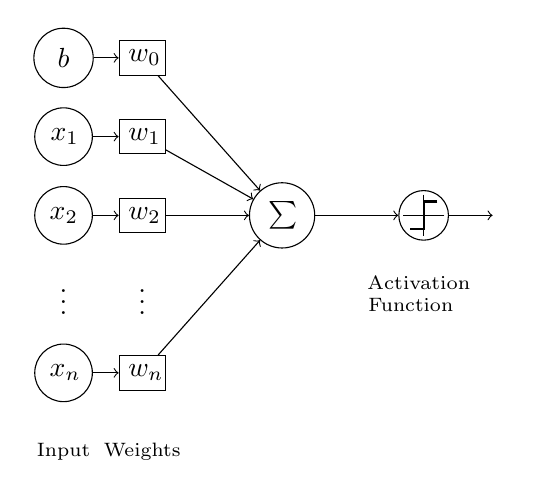
\begin{tikzpicture}
        \node[functions] (center) {};
        \node[below of=center,font=\scriptsize,text width=4em] {Activation Function};
        \draw[thick] (0.5em,0.5em) -- (0,0.5em) -- (0,-0.5em) -- (-0.5em,-0.5em);
        \draw (0em,0.75em) -- (0em,-0.75em);
        \draw (0.75em,0em) -- (-0.75em,0em);
        \node[right of=center] (right) {};
            \path[draw,->] (center) -- (right);
        \node[functions,left=3em of center] (left) {$\sum$};
            \path[draw,->] (left) -- (center);
        \node[weights,left=3em of left] (2) {$w_2$} -- (2) node[input,left of=2] (l2) {$x_2$};
            \path[draw,->] (l2) -- (2);
            \path[draw,->] (2) -- (left);
        \node[below of=2] (dots) {$\vdots$} -- (dots) node[left of=dots] (ldots) {$\vdots$};
        \node[weights,below of=dots] (n) {$w_n$} -- (n) node[input,left of=n] (ln) {$x_n$};
            \path[draw,->] (ln) -- (n);
            \path[draw,->] (n) -- (left);
        \node[weights,above of=2] (1) {$w_1$} -- (1) node[input,left of=1] (l1) {$x_1$};
            \path[draw,->] (l1) -- (1);
            \path[draw,->] (1) -- (left);
        \node[weights,above of=1] (0) {$w_0$} -- (0) node[input,left of=0] (l0) {$b$};
            \path[draw,->] (l0) -- (0);
            \path[draw,->] (0) -- (left);
        \node[below of=ln,font=\scriptsize] {Input};
        \node[below of=n,font=\scriptsize] {Weights};
    \end{tikzpicture}
\caption{Single Perceptron Unit}
\end{figure}

From the figure above, we have that $\{x_1,...,x_n\}$ form our input vector(note that $n$ can be very high dimensional) and we also introduce a bias term $b$. This bias term ensures that we are not restricted to hyperplanes that pass through 0 by taking only linear combinations $w_1x_1 +...+ w_nx_n$, but also to define affine transforms to shift the hyperplane. The weight vector $\{w_0, ..., w_n\}$ are the parameters of the perceptron and also the weights or importance assigned to each input. While simple, this perceptron allows us to express not just linear decision boundaries, but also non-linearly separable data.\\

But even thought it is able to represent some non-linear data, much of the complex data points still cannot be represented by a perceptron due to it's simplicity. This is because the \textit{linear function} $\sum = w_1x_1 + ... + w_nx_n$ is actually a linear combination of inputs with respect to the weights, and no matter how many layers of perceptrons are composed and connected together, \textbf{a linear combination of linear combinations is still a linear combination} which is an important property in linear algebra. Therefore in order to provide a way to express non-linear and complex data, we introduce the \textbf{activation function}.\\

\begin{figure}[!htb]
\centering
  \includegraphics[width=120mm]{activation.png}
  \caption{Common Activation Functions}
  \label{fig:af}
\end{figure}
 
The activation $f$ is a function that takes in our inputs, or more specifically, the result of the linear function $\sum = w_1x_1 + ... + w_nx_n$, as input and outputs a value. This adds a layer of complexity to the perceptron because now we are able to obtain non-linear function values from our input using the activation function we define. The simplest activation function is that of the step function(as seen in the perceptron figure) which outputs 1 if $\sum > 0$ else 0, but more commonly in CNNs Rectified Linear Unit(ReLU) are used. Others like sigmoid and $\tanh$ are also common choices.

\subsubsection{Gradient Descent}

Just as we do not wish to tweak the parameter weights ourselves, the perceptron is also able to learn the weights base on the output and actual label(ground truth) using \textbf{gradient descent}. This method of hill climbing to find the minima is also widely used in various learning based models like SVMs. First, let us define the loss function$L(w)$ that we wish to minimize. Then, we know that the minima of the loss function $L$ occurs when the derivative is 0.

\begin{equation*}
\triangledown L(w) = [\frac{\delta L}{\delta w_0}, \frac{\delta L}{\delta w_1}, ..., \frac{\delta L}{\delta w_n}] = 0
\end{equation*}

Also, we know that the gradient vector $\triangledown L$ points in the direction of the steepest ascent. Hence to climb \textit{down} the loss curve, we proceed in the opposite direction of the gradient vector by subtracting it.

\begin{equation*}
w' \rightarrow w + \triangle w \text{\ where } \triangle w =  - \eta \triangledown L(w)
\end{equation*}

where $\eta$ is the learning rate. This can also be shown to converge to the local minima given small enough value of $\eta$ and large enough training sample size using the Probably Approximately Correct (PAC) framework(details omitted).

\subsection{Multilayer Perceptron}

In essence, we can combine multiple perceptrons to form a single layer, and again formulate multiple layers and combine those layers to form a multilayer perceptron, which is a feedforward artificial neural network. This also describes the collection of fully connected layers that are placed in a CNN. Using this multilayer perceptron, we can output decision class(es) by using our fully connected layers to represent images or filter responses as a feature vector, and feed them forward to classify them. Previously, we have discussed the gradient descent method for a single perceptron. But what about learning the weights for multiple perceptrons? Because of the convoluted nature of feedforward networks, we cannot simply isolate perceptrons and calculate it's error, as error made by other perceptrons could have also influenced. Hence, we apply a higher level algorithm that uses gradient descent, known as backpropagation.

\subsubsection{Backpropagation Algorithm}

After feeding the input into the fully connected layers, and churning out the output, we start from the output and calculate the error for each layer and perceptron from the last layer to the front. That is, we propagate the error backward from the output. Let us define our activation function $o_k(\Sigma)$ that accepts our linear function as input, and outputs a single value for the $k^{th}$ output layer. For example, in the case of the sigmoid function:

\begin{equation*}
o_k(\Sigma) = \frac{1}{1 + \exp(\Sigma)}, \text{ where } \Sigma = w_1x_1 + ... + w_nx_n
\end{equation*}

Then, we wish to find the change in the weights $w_i$ for each of the output neuron such that the loss function$L(o)$ is minimized; That is we wish to proceed in the opposite direction of the gradient vector $\frac{\delta L}{\delta w_i}$. More specifically for the output layer, let us define $w_{hk}$ be the weight assigned to the input from the $h^{th}$ hidden layer neuron, to the $k^{th}$ output layer neuron. Then, we wish to find:

\begin{equation*}
\triangle w_{hk} = -\eta \frac{\delta L}{\delta w_{hk}} = - \eta  \frac{\delta L}{\delta o_k} \frac{\delta o_k}{\delta \Sigma_k} \frac{\delta \Sigma_k}{\delta w_{hk}} 
\end{equation*}

where we used the Chain Rule from Calculus to decompose the gradient formulation into equations we can derive easily. Using the example where the activation function is sigmoid, we have:
\begin{equation*}
\frac{\delta L}{\delta o_k} = \frac{\delta }{\delta o_k} \frac{1}{2} \sum_{k' \in K} (y_{k'} - o_{k'})^2  = - (y_k - o_k)
\end{equation*}
 
\begin{equation*}
 \frac{\delta o_k}{\delta \Sigma_k} =  \frac{\delta}{\delta \Sigma_k} ( \frac{1}{1 + \exp(\Sigma_k)}) = o_k(\Sigma_k))
\end{equation*}

\begin{equation*}
 \frac{\delta \Sigma_k}{\delta w_{hk}} =   \frac{\delta }{\delta w_{hk}} (\sum_{h'} w_{h'k} o_{h'}) = o_h
\end{equation*}

Finally, we have that:
\begin{equation*}
\triangle w_{hk} = -\eta \frac{\delta L}{\delta w_{hk}} = - \eta  \frac{\delta L}{\delta o_k} \frac{\delta o_k}{\delta \Sigma_k} \frac{\delta \Sigma_k}{\delta w_{hk}} = \eta (y_k - o_k)o_k(1 - o_k)o_h
\end{equation*}

In the case of the hidden layer, the formulation is exactly the same, replacing with the appropriate variables, we have that for the weight connecting the input from the $i^{th}$ neuron in the previous layer to the $h^{th}$ neuron in the current hidden layer:
\begin{equation*}
\triangle w_{ih} = -\eta \frac{\delta L}{\delta w_{ih}} = - \eta  \frac{\delta L}{\delta o_h} \frac{\delta o_h}{\delta \Sigma_k} \frac{\delta \Sigma_k}{\delta w_{ih}} 
\end{equation*}

The main issue here is in the first term, $ \frac{\delta L}{\delta o_h}$. Previously, we were able to compute  $\frac{\delta L}{\delta o_k}$ by comparing the ground truth labels $y_k$ with the output value $o_k$. But in the case of the hidden layer, there is no ground truth label to compare the output $o_h$ with. For each hidden layer neuron, the value of that neuron implicitly contributes to the value of  each of the output layer neurons through feedforward phase. Hence, we need to estimate the loss contribution of this hidden neuron by aggregating the total loss contributed in later hidden layers and the output layer by this hidden neuron. That is,

\begin{equation*}
\frac{\delta L}{\delta o_h} = \sum_{k \in K} \frac{\delta L}{\delta o_k} \frac{\delta o_k}{\delta \Sigma_k} \frac{\delta \Sigma_k}{\delta o_h} 
\end{equation*}

For the hidden layer before the output layer. In general if we wish the find the changes in weight $w_i$ going from the $j$ hidden layer to the $j + 1$ hidden layer with $H'$ units, then:
 
\begin{equation*}
\frac{\delta L}{\delta o_{h^{(j)}}} = \sum_{h' \in H'} \frac{\delta L}{\delta o_{h'^{(j+1)}}} \frac{\delta o_{h'^{(j+1)}}}{\delta \Sigma_{h'^{(j+1)}}} \frac{\delta \Sigma_{h'^{(j+1)}}}{\delta o_{h'^{(j+1)}}} 
\end{equation*}

To summarise, we perform the feedforward step to obtain the output layer values so that we can compute the loss function $L$ using our output values. Then, we iteratively backpropagate the loss and change the weights accordingly by using the loss computed from the previous layer from the back.

\subsubsection{Backpropagation for Convolutonal Layer}

The backpropagation algorithm for the convolutional layer is similar to the standard backpropagation algorithm, except that now we deal with pixels in the feature map as input. Without going too much into detail, let us take the pixel output from the previous layer $l - 1$ as $o^{(l - 1)}_{i, j}$, the convolved pixel at the current layer $x^{(l)}_{i,j}$ and the output from the activation function using this convolved pixel at the $l$ layer as $o^{(l)}_{i,j}$. Then, the convolution operation at layer $l$ is represented as:

\begin{equation*}
x^{(l)}_{i,j} = \sum_m \sum_n w^{(l)}_{m, n} o^{(l - 1)}_{i-m, j-n} + b^{(l)}_{i, j}
\end{equation*}
\begin{equation*}
o^{(l)}_{i,j} = o(x^{(l)}_{i,j})
\end{equation*}

For a $k_1 \times k_2$ kernel and an input feature map/image of $H \times W$, the convolution operation produces a feature map with dimensions $(H - k_1 + 1) \times (W - k_2 + 1)$ Then the gradient component can be computed as such:

\begin{flalign}
\begin{aligned}
\frac{\delta L}{\delta w^{(l)}_{m, n}} &= \sum_{i = 0}^{H - k_1} \sum_{j = 0}^{w - k_2} \frac{\delta L}{\delta o^{(l)}_{i,j}} \frac{\delta o^{(l)}_{i,j}}{\delta x^{(l)}_{i,j}} \frac{\delta  x^{(l)}_{i,j}}{\delta w^{(l)}_{m, n}} 
\end{aligned}
\end{flalign}

where $\frac{\delta L}{\delta o^{(l)}_{i,j}} \text{ and } \frac{\delta o^{(l)}_{i,j}}{\delta x^{(l)}_{i,j}}$  are computed in similar fashion to the standard backpropagation. We have that the last term:

\begin{flalign}
\begin{aligned}
 \frac{\delta  x^l_{i,j}}{\delta w^l_{m, n}} &=  \frac{\delta }{\delta w^l_{m, n}} ( \sum_m \sum_n w^l_{m, n} o^{(l - 1)}_{i-m, j-n} + b^{(l)}_{i, j}) \\
 &= \frac{\delta }{\delta w^l_{m, n}} (w^{(l)}_{m, n} o^{(l - 1)}_{i-m, j-n}) \\
 &=  o^{(l - 1)}_{i+m, j+n}
\end{aligned}
\end{flalign}

Hence, we finally have that:
\begin{flalign}
\begin{aligned}
\frac{\delta L}{\delta w^{(l)}_{m, n}} &= \sum_{i = 0}^{H - k_1} \sum_{j = 0}^{w - k_2} \frac{\delta L}{\delta o^{(l)}_{i,j}} \frac{\delta o^{(l)}_{i,j}}{\delta x^{(l)}_{i,j}} \frac{\delta  x^{(l)}_{i,j}}{\delta w^{(l)}_{m, n}} \\
&=  \sum_{i = 0}^{H - k_1} \sum_{j = 0}^{w - k_2} \frac{\delta L}{\delta o^{(l)}_{i,j}} \frac{\delta o^{(l)}_{i,j}}{\delta x^{(l)}_{i,j}} o^{(l - 1)}_{i-m, j-n}\\
&= [ \frac{\delta L}{\delta o^{(l)}_{i,j}} \times \frac{\delta o^{(l)}_{i,j}}{\delta x^{(l)}_{i,j}}]\ *\ o^{(l - 1)}_{m, n} \text{ where $\times$ is the Hadamard product}
\end{aligned}
\end{flalign}


\subsection{Properties of Convolutional Layers}

\subsubsection{Locality Based Processing}

We have taken a look at dense layers, and see how much more expressive it can be compared to convolutional layers where a set of filters are applied to the entire image, whereas dense layers are able to operate on pixels independently. Wouldn't we want to use fully connected layers instead for it's expressiveness? Again we go back to the first sections where we mentioned locality properties: where neighbouring pixels in a region often convey more information and cannot be ignored. Convolutional layers are to dense layers what filtering is to point processing. We want to be able to extract locality information information as well from a pixel, and hence convolutional layers play a big part in this. 

\subsubsection{Receptive Fields}

Similar to local features, using convolution layers to apply convolution operations using filters, we only extract local information for each window that may be isolated from information in other windows. This is also known as \textit{sparse interaction}. However, with enough filters in each layer, and sufficient convolutional layers, then the information extracted into feature maps are similar to channels in a colour image, and can expand to represent global information about the image. For example, if we perform edge detection, using simply a single derivative filter may not yield meaningful results. However, combining derivative filters in a single layer, along with gaussian smoothing in another may produce detections with smooth edges.

\subsubsection{Parameter Sharing}

Previously, we have briefly mentioned that in a convolutional layer, the 'weights' are shared in the form of filters, where the same set of filters are applied throughout the image instead of having different filters for different segments. This reduces the dimensionality of the parameters at this layer, but more importantly it \textit{preserves equivariant representation}. If the image is translated, then the output also changes accordingly.

\end{document}

